%This is a Latex file.
\documentclass[12pt]{article}
\usepackage{latexsym,fancyhdr,amsmath,amsfonts,amsthm,dsfont}
\usepackage{amssymb}
\usepackage{tikz}

% margins are relative to the default of 1 in
%\topmargin       -0.2 in

\topmargin        -0.2 in
\textheight       8.4 in
\oddsidemargin    0 in     % this is for pages 1, 3, 5, ...
\evensidemargin   0 in     % and this for 2, 4, 6, ...
\textwidth        6.5 in
%\headheight       15 in     % we won't have a running head, nor
\headsep          .35 in     % any extra space between head and text

%\parindent 0pt

\pagestyle{fancy} \lhead{\sf MTH 317} \chead{\sf Homework 1}
\rhead{\sf Rayana Gottschall} \lfoot{} \cfoot{} \rfoot{}

\newcommand{\C}{\mathds{C}}
\newcommand{\I}{\mathds{I}}
\newcommand{\N}{\mathds{N}}
\newcommand{\Q}{\mathds{Q}}
\newcommand{\R}{\mathds{R}}
\newcommand{\Z}{\mathds{Z}}

\begin{document}
\begin{enumerate}
\item[1.4] Let $S = \{-6, -3, 0, 3, 6\}$. Draw the graph $G$ whose vertex set is $S$ and such that $ij \in E(G)$ for $i, j \in S$ if $i + j \in S$ or $|i - j| \in S$.

\begin{center}
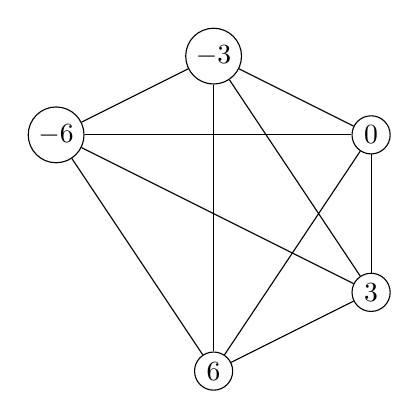
\begin{tikzpicture}[scale=1, every node/.style={circle, draw, fill=white, inner sep=2pt}]
    \node (A) at (0,2) {$-6$};
    \node (B) at (2,3) {$-3$};
    \node (C) at (4,2) {$0$};
    \node (D) at (4,0) {$3$};
    \node (E) at (2,-1) {$6$};

    \draw (A) -- (B);
    \draw (A) -- (C);
    \draw (A) -- (D);
    \draw (A) -- (E);
    \draw (B) -- (C);
    \draw (B) -- (D);
    \draw (B) -- (E);
    \draw (C) -- (D);
    \draw (C) -- (E);
    \draw (D) -- (E);
\end{tikzpicture}
\end{center}
    
 \item[1.15] Draw all connected graphs of order 5 in which the distance between every two distinct vertices is odd.  Justify your answer.
    \begin{center}
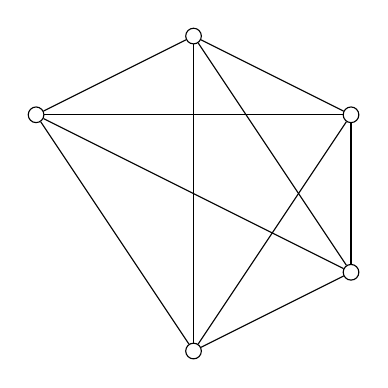
\begin{tikzpicture}[scale=1, every node/.style={circle, draw, fill=white, inner sep=2pt}]
    \node (A) at (0,2) {};
    \node (B) at (2,3) {};
    \node (C) at (4,2) {};
    \node (D) at (4,0) {};
    \node (E) at (2,-1) {};

    \draw (A) -- (B);
    \draw (A) -- (C);
    \draw (A) -- (D);
    \draw (A) -- (E);
    \draw (B) -- (C);
    \draw (B) -- (D);
    \draw (B) -- (E);
    \draw (C) -- (D);
    \draw (C) -- (E);
    \draw (D) -- (E);
\end{tikzpicture}
\end{center}
\noindent
This works because the graph is connected and the distance between any two vertices is 1, which is odd.  This is the only graph because if we remove any edge, the distance between some vertices will become 2.

\item[1.16]

\item[1.17]
\item[a] 
\item[b] 

\item[1.20 a)] What is the minimum size of a connected subgrpah of G containing u and v? 
\\
\noindent
By definition, d(u, v) is the shortest u-v path. A path is
a connected subgraph. Therefore, the minimum size of a connected subgraph of G containing u and v is 
d(u, v).



\end{enumerate}
\end{document}
